\documentclass[12pt, letter]{exam}
\usepackage[utf8]{inputenc}
\usepackage[T1]{fontenc}
\usepackage[spanish]{babel}
\usepackage[autostyle,spanish=mexican]{csquotes}
\usepackage{amsmath}
\usepackage{amsthm}
\usepackage{physics}
\usepackage{tikz}
\usepackage{float}
\usepackage{siunitx}
\usepackage{multicol}
\usepackage{enumitem}
\usepackage[left=2.00cm, right=2.00cm, top=2.00cm, 
     bottom=2.00cm]{geometry}
\usepackage{pdfpages}

% \renewcommand{\questionlabel}{\thequestion}
\decimalpoint

\setlength{\belowdisplayskip}{-0.5pt}

\usepackage{tasks}
\settasks{
    label=\Alph*), 
    label-align=left,
    item-indent={20pt}, 
    column-sep={4pt},
    label-width={16pt},
}

\sisetup{per-mode=symbol}
\footer{}{\thepage}{}

\begin{document}

\includepdf[pages=-]{Caratula_Examen_Parcial_04_PU_Fisica_3_01_Grupo_43.pdf}

\setcounter{page}{3}

\begin{center}
\textbf{Cada ejercicio vale 1 punto, incluidos los ejercicios de ejecución.}
\end{center}

\begin{questions}

    \section{(7 puntos) Movimiento circular.}

    \question Identifica de la siguiente figura los elementos del círculo.
    \begin{figure}[H]
        \centering
        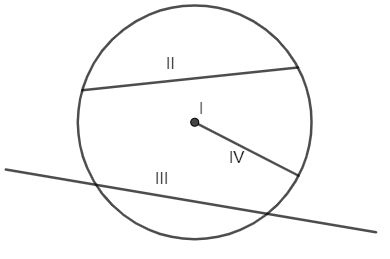
\includegraphics[scale=1]{Elementos_Circulo_01.png}
    \end{figure}
    \begin{multicols}{2}
    \begin{parts}
        \part Cuerda
        \part Radio
        \part Tangente
        \part Secante
        \part Centro
        \part Perímetro
    \end{parts}
    \end{multicols}
    
    \vspace*{0.25cm}
    Respuestas:
    \begin{multicols}{2}
    \begin{tasks}
        \task e-I, d-II, a-III, f-IV
        \task e-I, a-II, d-III, b-IV
        \task e-I, a-II, d-III, b-IV
        \task a-I, b-II, c-III, d-IV
    \end{tasks}
    \end{multicols}
    \question Considerando el radio (r), el radián se define como el ángulo central al que corresponde un arco de longitud igual: \rule{2cm}{0.1mm}.
    \begin{tasks}(4)
        \task $r$
        \task $\pi \, r$
        \task $2 \, r$
        \task $\dfrac{\pi}{2} \, r$
    \end{tasks}
    \question En el movimiento circular las unidades de frecuencia son: \rule{2cm}{0.1mm}
    \begin{tasks}(4)
        \task $\displaystyle \unit[per-mode=fraction]{\radian\per\second}$
        \task $\dfrac{1}{\unit{\second}}$
        \task $\displaystyle \unit[per-mode=fraction]{\meter\per\second}$
        \task $\displaystyle \unit[per-mode=fraction]{\radian\per\square\second}$
    \end{tasks}
    \question ¿Cuál es la trayectoria de la velocidad lineal de un objeto que describe un movimiento circular?
    \begin{tasks}(4)
        \task Una cuerda.
        \task Una secante.
        \task Un radio.
        \task Una tangente.
    \end{tasks}
    \question \label{Ejercicio_01} \textbf{Ejercicio de ejecución: } Convierte 2.18 radianes a grados.
    \begin{tasks}(4)
        \task \ang{100.47}
        \task \ang{124.90}
        \task \ang{249.80}
        \task \ang{392.40}
    \end{tasks}
    \question \label{Ejercicio_02} \textbf{Ejercicio de ejecución: } Un ventilador gira a de 900 rpm (rev/min). Determina la velocidad tangencial del extremo del aspa, si la distancia desde el centro al extremo es de \SI{20.0}{\centi\meter}.
    \begin{tasks}(4)
        \task \SI{12.9}{\meter\per\second}
        \task \SI{17.4}{\meter\per\second}
        \task \SI{18.8}{\meter\per\second}
        \task \SI{29.5}{\meter\per\second}
    \end{tasks}
    \question \label{Ejercicio_03} \textbf{Ejercicio de ejecución: } Una centrifugadora acelera desde el reposo hasta 20,000 rpm en \SI{30}{\second} ¿Cuál es su aceleración angular?
    \begin{tasks}(4)
        \task $\displaystyle \SI[per-mode=fraction]{69.81}{\radian\per\square\second}$
        \task $\displaystyle \SI[per-mode=fraction]{100.43}{\radian\per\square\second}$
        \task $\displaystyle \SI[per-mode=fraction]{210.04}{\radian\per\square\second}$
        \task $\displaystyle \SI[per-mode=fraction]{350.18}{\radian\per\square\second}$
    \end{tasks}

    \section{(4 puntos) Piezoelectricidad.}

    \question La piezoelectricidad es un fenómeno físico en el cual ciertos materiales tienen la capacidad de generar una \rule{2cm}{0.1mm} eléctrica.
    \begin{tasks}(4)
        \task Resistencia
        \task Carga
        \task Conductividad
        \task Potencia
    \end{tasks}
    \question Son materiales que presentan el efecto piezoeléctrico:
    \begin{multicols}{2}
    \begin{tasks}
        \task Cristales, Materia orgánica, Gases.
        \task Cristales, Líquidos, Cerámicos.
        \task Cristales, Cerámicos, Polímeros.
        \task Plásticos, Cerámicos, Polímeros.
    \end{tasks}
    \end{multicols}
    \question Una de las propiedades de los cerámicos es \rule{2cm}{0.1mm}

    \vspace{0.5cm}
    \begin{multicols}{2}
        \begin{tasks}
            \task Resistencia a la temperatura
            \task Alta conductividad eléctrica
            \task Alta Ductibilidad
            \task Alta Densidad
        \end{tasks}
    \end{multicols}
    \question En la transformación de energía mecánica a eléctrica en un material piezoeléctrico, al deformarse la estructura del material se genera: \rule{2cm}{0.1mm}
    \begin{tasks}(4)
        \task Resistencia
        \task Potencia
        \task Voltaje
        \task Fuerza
    \end{tasks}
    
    \section{(4 puntos) Superconductividad.}

    \question De la relación entre resistividad y conductividad sabemos que: a \rule{2cm}{0.1mm} sea la resistencia eléctrica de un material, \rule{2cm}{0.1mm} será su conductividad.
    \begin{tasks}(4)
        \task Mayor - Mayor
        \task Menor - Mayor
        \task Mayor - Menor
        \task Menor - Menor
    \end{tasks}
    \question Un material superconductor se caracteriza por que su resistencia interna \rule{2cm}{0.1mm}
    \begin{tasks}(4)
        \task Se incrementa.
        \task Vale cero.
        \task Se hace negativa.
        \task No cambia.
    \end{tasks}

    \newpage

    \question El valor de temperatura en el que se presenta el estado superconductor en un material, se le conoce como \rule{2cm}{0.1mm}
    \begin{multicols}{2}
    \begin{tasks}
        \task Temperatura crítica.
        \task Temperatura mínima.
        \task Temperatura máxima.
        \task Temperatura estándar.
    \end{tasks}
    \end{multicols}
    \question Una de las características de un material superconductor es que repele un campo magnético externo, lo que se conoce como efecto: \rule{2cm}{0.1mm}
    \begin{tasks}(4)
        \task Tesla
        \task Faraday
        \task Meissner
        \task Cherenkov
    \end{tasks}

    \section{(5 puntos) Sustentabilidad y contaminación.}

    \question Cuando nos referimos a la capacidad de satisfacer las necesidades actuales de la sociedad sin comprometer la capacidad de las futuras generaciones para satisfacer sus propias necesidades, hablamos de: \rule{2cm}{0.1mm}
    \begin{tasks}(4)
        \task Economía
        \task Sostenibilidad
        \task Crecimiento
        \task Sustentabilidad
    \end{tasks}
    \question Este fenómeno ocurre cuando ciertos gases en la atmósfera terrestre retienen el calor emitido por la Tierra y lo reenvían de vuelta a la superficie, lo que produce un aumento de la temperatura global: \rule{2cm}{0.1mm}
    \begin{tasks}(4)
        \task Efecto invernadero
        \task Inversión térmica
        \task Cambio climático
        \task Contaminación del aire
    \end{tasks}
    \question La Asamblea General de las Naciones Unidas en 2009 estableció el Día Internacional de la Madre Tierra, que se celebra el \rule{2cm}{0.1mm} de cada año como un recordatorio de la importancia de cuidar y proteger nuestro planeta.
    \begin{tasks}(4)
        \task 1 de mayo
        \task 22 de abril
        \task 9 de septiembre
        \task 4 de enero
    \end{tasks}
    \question La inversión térmica es un fenómeno que se presenta cuando la temperatura del aire \rule{2cm}{0.1mm} conforme subimos en altura.
    \begin{tasks}(4)
        \task Disminuye
        \task Aumenta
        \task No cambia
        \task Se equilibra
    \end{tasks}
    \question Las partículas PM10 son aquellas partículas sólidas o líquidas de diferente composición y tamaño que se encuentran dispersas en la atmósfera y que tienen un diámetro \rule{2cm}{0.1mm}
    \begin{tasks}(4)
        \task Mayor que \SI{10}{\micro\meter}
        \task Menor que \SI{10}{\micro\meter}
        \task Igual a \SI{0.1}{\micro\meter}
        \task Igual a \SI{0.01}{\micro\meter}
    \end{tasks}
\end{questions}

\newpage

\textbf{\huge{Formulario.}}
\begin{table}[H]
    \centering
    \setlength{\tabcolsep}{40pt}
    \renewcommand{\arraystretch}{2}
    \begin{tabular}{c  c}
        \multicolumn{2}{c}{Movimiento circular} \\
        \ang{360} = $2 \, \pi$ radianes & $T = \dfrac{\text{segundos transcurridos}}{\text{1 ciclo}}$ \\
        $f = \dfrac{\text{número de ciclos}}{\text{1 segundo}}$ & $\omega = \dfrac{\theta}{t}$ \\
        $\omega = \dfrac{\theta_{f} - \theta_{i}}{t_{f} - t_{i}}$ & $\omega = \dfrac{2 \, \pi \, \text{rad}}{T}$ \\
        $\omega = 2 \, \pi \, f $ & $\omega_{m} = \dfrac{\omega_{f} + \omega_{i}}{2}$ \\
        $v_{T} = \dfrac{2 \, \pi \, r}{T}$ & $v_{T} = \omega \cdot r$ \\
        $\alpha = \dfrac{\omega_{f} - \omega_{i}}{t_{f} - t_{i}}$ & $a_{c} = \dfrac{v_{T}^{2}}{r}$ \\
        $\theta = \dfrac{\omega_{f}^{2} - \omega_{i}^{2}}{2 \, \alpha}$ & $\theta = \omega_{i} \, t + \dfrac{\alpha \, t^{2}}{2}$ \\
        $\theta = \dfrac{\alpha \, t^{2}}{2}$ & $\theta = \dfrac{\omega_{f} + \omega_{i}}{2} \, t$ \\
        $\theta = \dfrac{\omega_{f}}{2} \, t$ & $\theta = \dfrac{\omega_{f}^{2}}{2 \, \alpha}$ \\
        $\omega_{f} = \omega_{i}^{2} + 2 \, \alpha \, \theta$ & $\omega_{f} = \omega_{i} + \alpha \, t$ \\
        $\omega_{f} = 2 \, \alpha \, \theta$ & $\omega_{f} = \alpha \, t$ \\ \hline
        
\end{tabular}
\end{table}

\newpage

En este espacio deberás de incluir el desarrollo completo de los Problemas de Ejecución. El problema se califica de la siguiente manera:
\begin{enumerate}[label=\alph*)]
\item \textbf{Datos:} 0.25 puntos.
\item \textbf{Expresión(es):} 0.25 puntos.
\item \textbf{Sustitución:} 0.25 puntos.
\item \textbf{Manejo de unidades:} 0.25 puntos.
\end{enumerate}

\vspace*{0.5cm}

Solución al Problema de Ejecución \ref{Ejercicio_01}:

\vspace*{4cm}
\rule{0.9\textwidth}{0.3mm}

Solución al Problema de Ejecución \ref{Ejercicio_02}:

\vspace*{4cm}
\rule{0.9\textwidth}{0.3mm}

Solución al Problema de Ejecución \ref{Ejercicio_03}:

\end{document}